\chapter{软件需求规格说明书}
\section{引言}
需求文档描述软件需求,主要用于明确系统需要实现的功能、性能、接口、设计约束等,
确保开发团队与客户对项目需求有一致的理解。为开发团队提供需求指导,并作为后续开发、测试、验收的重要参考。
\section{功能需求}

\subsection{管理人员需求}
\begin{itemize}
    \item{商家使用}:商家能够注册并向平台提供自己的店铺信息,注册店铺。
    \item{用户使用}:用户可以注册登录,进行下单。
\end{itemize}


\subsection{用户需求}
\subsubsection{普通用户需求}
\begin{itemize}
    \item{下单流畅}:使用时应该流畅,能够随时中断,随时返回到上一页面以及返回主页等页面。并且在订单未支付时候返回,应该保留历史订单,之后支付。
    \item{购物透明}:能够随时看到自己已经购入了什么,需要花费多少;正确显示历史购买记录。
    \item {搜索功能}:可以搜索到相关商家。
    \item {修改个人信息}:可以修改个人信息,地址。
\end{itemize}

\subsubsection{商家用户需求}
\begin{itemize}
    \item {调整商品}:可以上架商品,删除商品,修改商品信息。
    \item{修改商家信息}:可以修改商家的信息。
\end{itemize}

\section{非功能需求}
可以正确显示页面。

\section{UML图}
注册与登录如图
\begin{figure}[htbp]
    \centering
    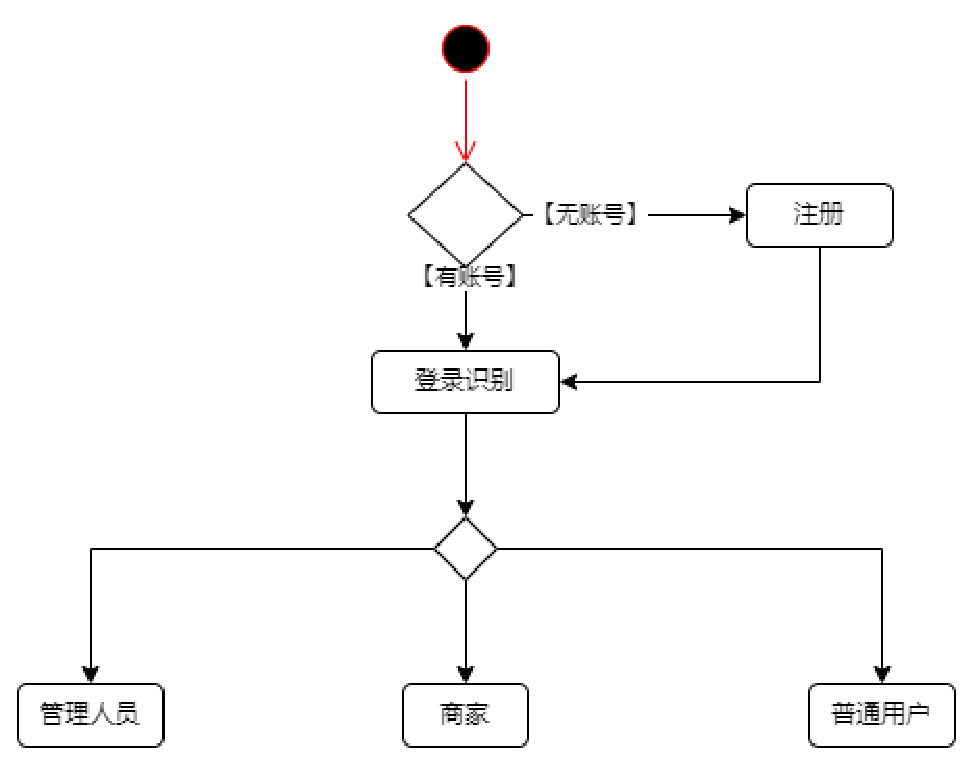
\includegraphics[width=1\textwidth]{login}
    \caption{注册与登录活动图}\label{fig:ds}
\end{figure}

用户如何成为商家如图\ref{fig:dd}
\begin{figure}[htbp]
    \centering
    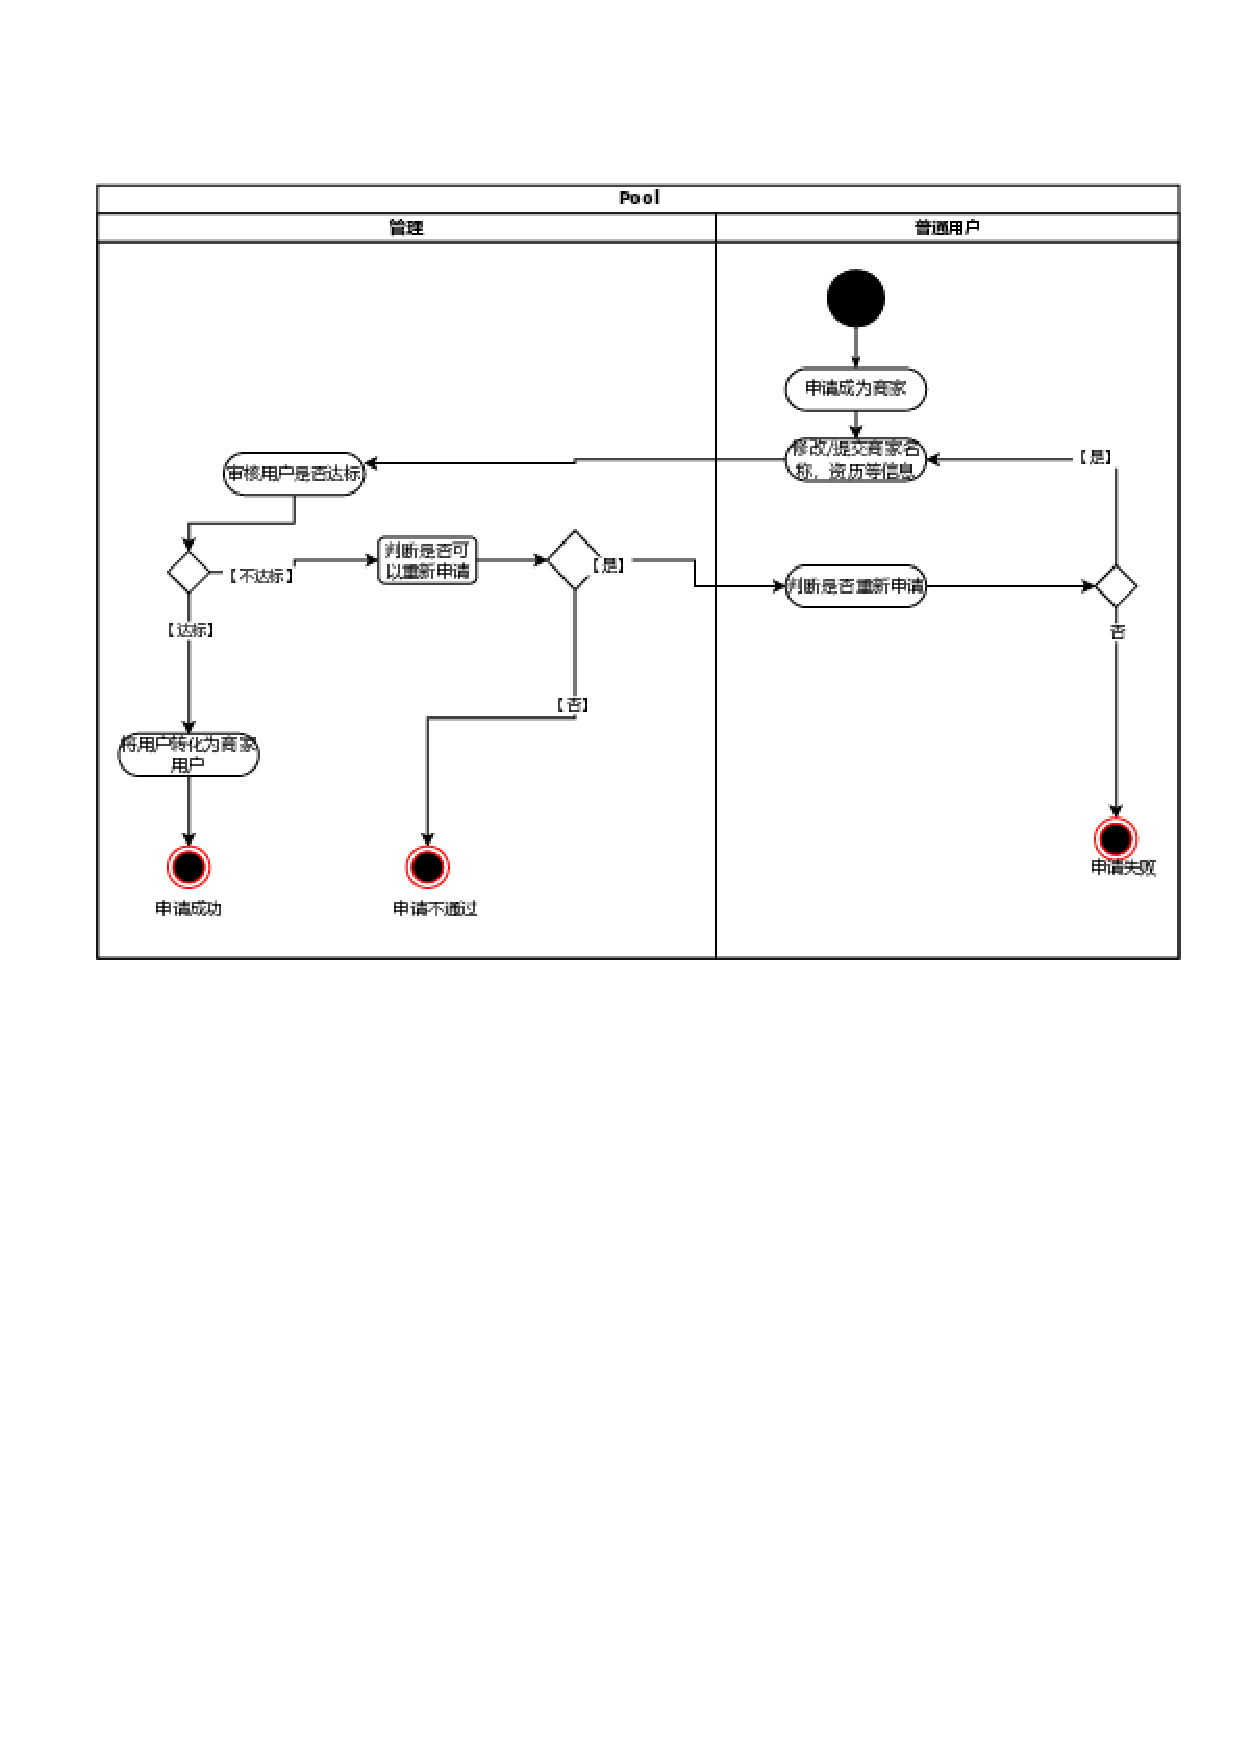
\includegraphics[width=1\textwidth]{utobe}
    \caption{用户转化为商家}\label{fig:dd}
\end{figure}
